\section{Engineering aspects}\label{sec-engineering}

In the previous sections we have modelled the most critical subset of various
build systems. However, like all real-world systems, there are many corners that
obscure the essence. In this section we discuss some of those details, what
would need to be done to capture them in our model, and what the impact would be.

\subsection{Partial Stores and Exceptions}

Our model assumes a world where the store is fully-defined, every \hs{k} is
associated with a \hs{v}, and every compute successfully completes returning a
valid value. In the real world, build systems frequently deal with errors, e.g.
``file not found'' or ``compilation failed''. We can model such failure
conditions by instantiating \hs{v} to either \hs{Maybe}~\hs{v} (for missing
values) or \hs{Either}~\hs{e}~\hs{v} (for exceptions of type \hs{e}). That can
model the errors inside the store and the \hs{Task}, but because \hs{v} is
polymorphic for builds, it does not let the build system apply special behaviour
for errors, e.g. early aborting.

\subsection{Parallelism}\label{sec-parallelism}

We have given simple implementations assuming a single thread of execution,
but all the build systems we address can actually build independent keys in parallel.
While it complicates the model, the complications can be restricted exclusively
to the scheduler:

\begin{enumerate}
\item The \hs{topological} scheduler can build the full dependency graph, and
whenever all dependencies of a task are complete, the task itself can be
started.

\item The \hs{restarting} scheduler can be made parallel in a few ways, but the
most direct is to have $n$ threads reading keys from the build queue. As before,
if a key requires a dependency not yet built, it is moved to the end~--~the
difference is that sometimes keys will be moved to the back of the queue not
because they are out of date but because of races with earlier tasks that had
not yet finished. As a consequence, over successive runs, potentially racey
dependencies will be separated, giving better parallelism over time.

\item The \hs{suspending} scheduler can be made parallel by starting static
dependencies of a \hs{Task} in parallel, while dynamic dependencies are being
resolved, using the strategy described by~\citet{marlow2014haxl}.
\end{enumerate}

The actual implementation of the parallel schedulers is not overly onerous,
but neither is it beautiful or informative.

\subsection{Impure Computations}\label{sec-non-determinism}

In our model we define \hs{Task} as a function -- when given the same inputs
it will always produce the same output. Alas, the real-world is not so obliging.
Some examples of impure tasks include:

\begin{description}
\item[Untracked dependencies] Some tasks depend on untracked values -- for example
C compilation will explicitly list the \cmd{source.c} file as a dependency,
but it may not record that the version of \cmd{gcc} is also a dependency.

\item[Non-determinism] Some tasks are \emph{non-deterministic}, producing a
result from a possible set. As an example, GHC when compiled using parallelism
can change the order in which unique variables are obtained from the supply,
producing different but semantically identical results.

\item[Volatility] Some tasks are defined to change in every build, e.g. \Excel
provides a~``function'' \cmd{RANDBETWEEN} producing a fresh random number in a
specified range on each recalculation. Similarly, build systems like \Make and
\Shake provide volatile \emph{phony rules}. The main difference from
non-deterministic tasks is that volatile tasks cannot be cached. They are best
modelled as depending on a special key \cmd{RealWorld} whose value is changed
in every build.
\end{description}

Interestingly, there is significant interplay between all three sources of
impurity. Systems like \Bazel use various sandboxing techniques to guard against
missing dependencies, but none are likely to capture all dependencies right down
to the CPU model and microcode version. Tasks that do have untracked
dependencies can be marked as volatile, a technique \Excel takes with the
\cmd{INDIRECT} function, removing the untracked dependency at the cost of
minimality.

Most of the implementations in \S\ref{sec-implementations} can deal with
non-determinism, apart from \Buck, which relies on deterministic tasks, and
in turn can optimise the number of roundtrips required to the server.

One tempting way of modelling non-determinism is to enrich \hs{Tasks} from
\hs{Applicative} or \hs{Monad} to \hs{Alternative} or \hs{MonadPlus},
respectively. More concretely, the following task description corresponds to
a spreadsheet with the formula \cmd{B1 = A1 + RANDBETWEEN(1,2)}.

\begin{minted}[xleftmargin=10pt]{haskell}
sprsh3 :: Tasks MonadPlus String Integer
sprsh3 "B1"@\,@=@\,@Just $ Task $ \fetch -> (+) <$> fetch "A1" <*> (pure@\,@1 <|> pure@\,@2)
sprsh3 _   @\,@=@\,@Nothing
\end{minted}
\vspace{1mm}

\noindent
Such tasks can be modelled in our framework by adjusting the correctness
definition (\S\ref{sec-build-correctness}): instead of requiring that the
\hs{result}ing value \emph{equals} the one obtained by recomputing the \hs{task}:
\[
\hs{getValue}~\hs{k}~\hs{result}~\hs{==}~\hs{compute}~\hs{task}~\hs{result}\text{,}
\]
\noindent
we now require that \hs{result} contains \emph{one possible result of
recomputing} the \hs{task}:
\[
\hs{getValue}~\hs{k}~\hs{result}~\hs{`elem`}~\hs{computeND}~\hs{task}~\hs{result}\text{,}
\]
where
\hs{computeND}~\hs{::}~\hs{Task}~\hs{MonadPlus}~\hs{k}~\hs{v}~\hs{->}~\hs{Store}~\hs{i}~\hs{k}~\hs{v}~\hs{->}~\hs{[@@v]}
returns the list of all possible results of the \hs{task} instead of just one
value (`ND' stands for `non-deterministic').

Note that \hs{Task}~\hs{MonadPlus} is powerful enough to model dependency-level
non-determinism, for example, \cmd{INDIRECT("A" \& RANDBETWEEN(1,2))}, whereas
most build tasks in real-life build systems only experience a value-level
non-determinism. \Excel handles this example simply by marking the cell
volatile~--~an approach that can be readily adopted by any of our
implementations.

\subsection{Cloud Implementation}\label{sec-cloud-aspects}

Our model of cloud builds provides a basic framework to discuss and reason
about them, but lacks a number of important engineering corners:

\begin{description}
\item[Communication] When traces or contents are stored in the cloud,
communication can become a bottleneck, so it is important to send only the
minimum amount of information, optimising with respect to build system
invariants. For example, incremental data processing systems in the cloud, such
as \Reflow~\cite{reflow}, need to efficiently orchestrate terabytes of data.

\item[Offloading] Once the cloud is storing build products and traces, it is
possible for the cloud to also contain dedicated workers that can execute tasks
remotely~--~offloading some of the computation and potentially running vastly
more commands in parallel.

\item[Eviction] The cloud storage, as modelled
in~\S\ref{sec-constructive-traces}, grows indefinitely, but often resource
constraints require evicting old items from the store. When evicting an old
value \hs{v}, one can also evict all traces mentioning the now-defunct
\hs{hash}~\hs{v}. However, for shallow builds (see below), it is beneficial to
keep these traces, allowing builds to ``pass-through'' hashes whose underlying
values are not known, recreating them only when they must be materialised.

\item[Shallow builds] Building the end result, e.g. an installer package, often
involves many intermediate tasks. The intermediate results may be large, so some
cloud build systems are designed to build end products \emph{without
materialising} intermediate results, producing a so-called \emph{shallow build}
(see an example in~\S\ref{sec-background-bazel}). Some build systems go even
further, integrating with the file system to only materialise the file when the
user accesses it \cite{gvfs}.
\end{description}

To legitimise shallow builds, we need to relax the correctness
Definition~\ref{def-correct} as follows. Let the \hs{shallow} store correspond
to the result of a shallow build. Then \hs{shallow} is correct, if \emph{there
exists} a \hs{result} which satisfies all requirements of the
Definition~\ref{def-correct}, \emph{such that} \hs{shallow} agrees with the
\hs{result} on all the input keys \hs{k}~$\in$~$I$:
\[
\hs{getValue}~\hs{k}~\hs{shallow}~\hs{==}~\hs{getValue}~\hs{k}~\hs{result}\text{,}
\]
and on the target \hs{key}:
\[
\hs{getValue}~\hs{key}~\hs{shallow}~\hs{==}~\hs{getValue}~\hs{key}~\hs{result}\text{.}
\]

\noindent
This relaxes the requirements on shallow builds by dropping the constraints on
the \hs{shallow} store for all intermediate keys \hs{k}~$\in$~$O\setminus \{\hs{key}\}$.

\begin{figure}
\begin{subfigure}[b]{0.32\linewidth}
\centerline{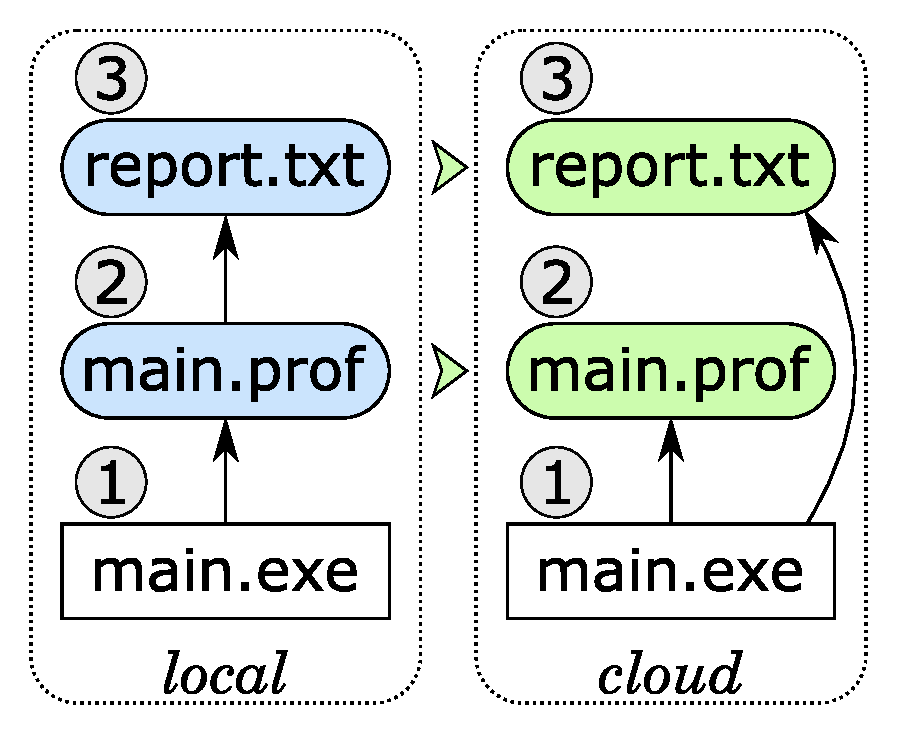
\includegraphics[scale=0.28]{fig/frankenbuild-example-build.pdf}}
\vspace{-1.5mm}
\caption{Initial build}
\end{subfigure}
\begin{subfigure}[b]{0.32\linewidth}
\centerline{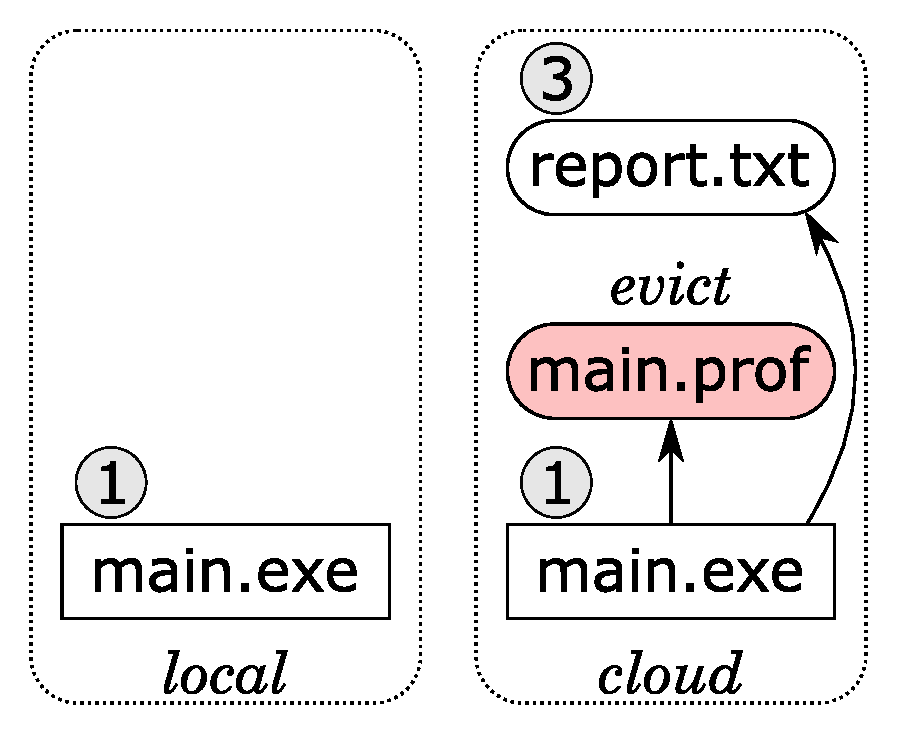
\includegraphics[scale=0.28]{fig/frankenbuild-example-clean.pdf}}
\vspace{-1.5mm}
\caption{Clean up and evict \cmd{main.prof}}
\end{subfigure}
\begin{subfigure}[b]{0.34\linewidth}
\centerline{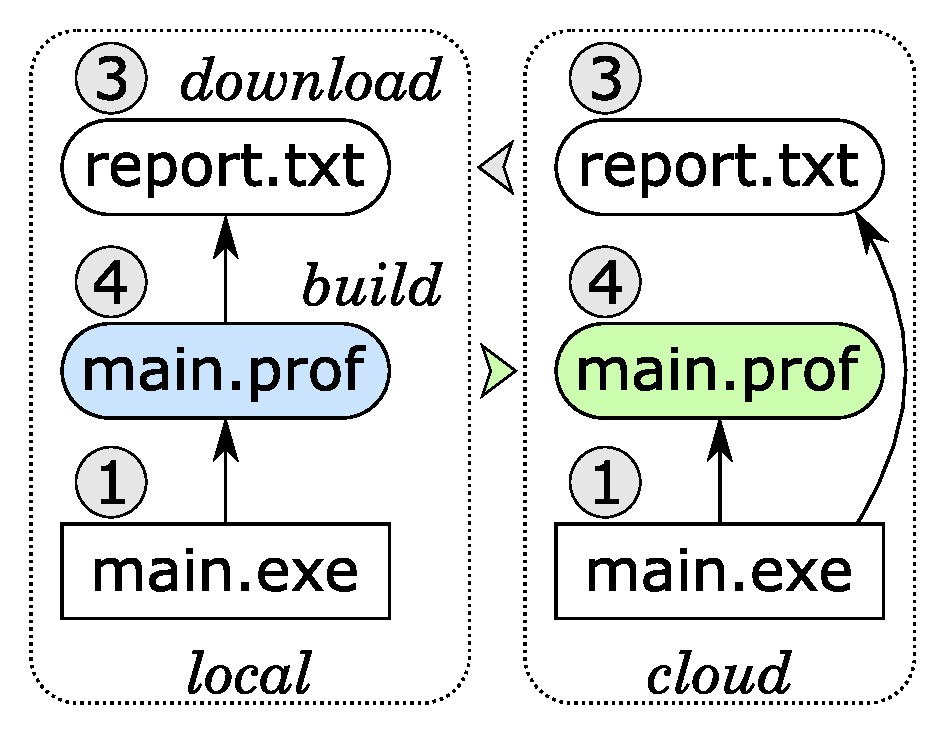
\includegraphics[scale=0.28]{fig/frankenbuild-example-rebuild.pdf}}
\vspace{-1.5mm}
\caption{Build \cmd{main.prof} and \cmd{report.txt}}
\end{subfigure}
\vspace{-1.5mm}
\caption{A Frankenbuild example: (a)~build a human-readable profiling report for
\cmd{main.exe} from information dump \cmd{main.prof} produced by a profiling
tool, then record deep constructive traces in the cloud, (b)~remove built files
locally and evict \cmd{main.prof} from the cloud storage, (c)~build
\cmd{main.prof} by executing the profiler (profiling is non-deterministic, hence
the new hash value), then build \cmd{report.txt} by downloading it from the
matching deep constructive trace in the cloud, resulting in a Frankenbuild
because \cmd{main.prof} and \cmd{report.txt} are inconsistent. New and evicted
cloud storage entries are highlighted; file hashes are shown in circles.
\label{fig-frankenbuild}}
\vspace{-4mm}
\end{figure}

Deep constructive traces (\S\ref{sec-deep-constructive-traces}) combined with
task non-determinism (\S\ref{sec-non-determinism}) can lead to very subtle bugs,
especially in the cloud setting. Fig.~\ref{fig-frankenbuild} shows a
\emph{Frankenbuild}~\cite{esfahani2016cloudbuild} example, where the target
\cmd{report.txt}, which is downloaded from the cloud, is inconsistent with its
immediate dependency \cmd{main.prof}. This inconsistency is caused by two factors:
(i)~inherent non-determinism of profiling: running a profiling tool on the very
same \cmd{main.exe} will produce different \cmd{main.prof} results every time;
and (ii)~relying on deep constructive traces, which cache build results based
only on the hashes of terminal task inputs (in this case \cmd{main.exe}). Note
that the resulting store is incorrect according to all three definitions of
correctness: the main definition~(\S\ref{sec-build-correctness}), the variant
for non-deterministic tasks~(\S\ref{sec-non-determinism}) and the variant for
shallow builds~(this section).

\subsection{Self-tracking}\label{sec-tracking-aspects}

Some build systems, for example \Excel and \Ninja, are capable of recomputing a
task if either its dependencies change, \emph{or} the task itself changes. For
example:

\vspace{0.5mm}
\begin{minted}[xleftmargin=10pt]{text}
A1 = 20      B1 = A1 + A2
A2 = 10
\end{minted}
\vspace{0.5mm}

\noindent
In \Excel the user can alter the value produced by \cmd{B1} by either editing
the inputs of \cmd{A1} or \cmd{A2}, \emph{or} editing the formula in
\cmd{B1}~--~e.g. to \cmd{A1 * A2}. This pattern can be captured by describing
the rule producing \cmd{B1} as also depending on the value \cmd{B1-formula}.
The implementation can be given very directly in a
\hs{Tasks}~\hs{Monad}~--~concretely, first look up the formula, then interpret
it:

\vspace{0.5mm}
\begin{minted}[xleftmargin=10pt]{haskell}
sprsh4 "B1" = Just $ Task $ \fetch -> do
    formula <- fetch "B1-formula"
    evalFormula fetch formula
\end{minted}
\vspace{0.5mm}

\noindent
The build systems that have precise self-tracking are all ones which use a
\emph{non-embedded domain specific language} to describe build tasks. Those
which use a full programming language, e.g. \Shake, are faced with the challenge
of implementing equality on arbitrary task functions. For such build systems,
the pessimistic assumption that any change to the build system potentially
changes any build task can often be used~--~the classic example being a makefile
depending on itself.

\subsection{Iterative Computations}\label{sec-iterative-compute}

Some computations are best described not by a chain of acyclic dependencies,
but by a loop. For example, \LaTeX~requires repeated rebuilding until it
reaches a fixed point, which can be directly expressed in build systems, such as
\Pluto~\cite{erdweg2015pluto}. Another example is \Excel, where a cell can
depend on itself, for example: \cmd{A1 = A1 + 1}. In such cases \Excel will
normally not execute anything, but if the ``Iterative Calculations'' feature is
enabled \Excel will execute the formula for a specified maximum number $N$ of
times per calculation (where $N$ is a setting that defaults to 100).

For examples like \LaTeX~we consider the proper encoding to not be circular
tasks, but a series of iterative steps, as described
by~\citet{shake-fixed-point}. It is important that the number of executions is
bounded, otherwise the build system may not terminate (a legitimate concern
with \LaTeX, which can be put into a situation where it is bistable or diverging
over multiple executions). The examples in \Excel tend to encode either mutable
state, or recurrence relations. The former is only required because \Excel
inherently lacks the ability to write mutable state, and the latter is probably
better solved using explicit recurrence formulae.

Overall we choose not to deal with cyclic dependencies, a choice that most build
systems also follow. There are computation frameworks that support tasks with
cyclic dependencies under the assumption that tasks are \emph{monotonic} in a
certain sense, e.g. see~\cite{pottier2009lazy} and~\cite{radul2009propagation}.

\subsection{Polymorphism}\label{sec-polymorphism}

Our build system abstraction assumes a \hs{k}/\hs{v} store, along with a build
system that works directly on \hs{k} and \hs{v} values. However, some build
systems provide greater flexibility, e.g. \Shake permits polymorphic keys and
values, allowing types that are stored only in the \Shake's build information.

As one example of richer key/value types, consider the version of
\cmd{gcc}~--~for many builds it should be a dependency. In \Shake it is possible
to define an \emph{oracle} rule as per~\cite{mitchell2012shake} whose value is
the result of running \cmd{gcc -}\cmd{-version} and which is volatile, making the
\cmd{gcc} version something that can be depended upon. Of course, provided the
build can express volatile dependencies and supports cutoff, the version number
could equally be written to a file and used in a similar way.

A more compelling example is build tasks that produce multiple output
keys~--~for example, \cmd{ghc Foo.hs} produces both \cmd{Foo.hi} and \cmd{Foo.o}.
That can be represented by having a key whose value is a pair of file names, and
whose result is a pair of file contents. From that, the task for \cmd{Foo.hi}
can be the first component of the result of the pair. Again, such an operation
can be encoded without polymorphic keys provided the pair of files (or a dummy
file representing the pair) is marked as changed if either of the contained
files change. Once again, polymorphic dependencies provide convenience rather
than power.

\Shake users have remarked that polymorphism provides a much easier expression
of concepts, e.g.~\cite{hadrian}, but it is not essential and we therefore do
not model it in this paper\footnote{See modules \cmd{Build.Multi} and
\cmd{Build.Task.Typed} in our framework for models of multiple-output and
polymorphic tasks.}.
